\documentclass[11pt]{article}
\usepackage[a4paper,margin=1.8cm]{geometry}
\usepackage[T1]{fontenc}
\usepackage{lmodern}
\usepackage{microtype}
\usepackage{booktabs}
\usepackage{graphicx}
\usepackage{amsmath}
\usepackage[hidelinks]{hyperref}

% Slightly tighter section and caption spacing (still readable).
\makeatletter
\renewcommand\section{\@startsection{section}{1}{\z@}%
  {-1.6ex \@plus -.5ex \@minus -.2ex}{0.8ex \@plus .2ex}{\normalfont\large\bfseries}}
\makeatother
\setlength{\parskip}{0pt}
\setlength{\abovecaptionskip}{4pt}
\setlength{\textfloatsep}{8pt plus 2pt minus 2pt}

\title{\vspace{-1.2cm}Do small open LLMs collude like humans?\\[2pt]
\large Repeated Bertrand markets with and without chat, after Fonseca \& Normann (2012)}
\author{Rodrigo Delgado, SPAR --- Learning dynamics in competitive multiagent environments%
\thanks{The text was drafted with Claude (Anthropic) from the project's results files and research notes.}}
\date{\vspace{-0.3cm}22 October 2026}

\begin{document}
\maketitle
\vspace{-0.9cm}

\begin{abstract}
\noindent
Open reasoning models under 30B parameters played the firms in one four-firm Bertrand market each, a NoTalk part then a surprise Talk part with free chat, as in Fonseca \& Normann.
With chat, all five 26--27B models reached and held the monopoly price of 100 (humans: 81.3), and four of them also sustained NoTalk prices far above the human 6.0; gpt-oss-20b, Qwen3-14B, Granite-4.2-8B and LFM-2.5-2.6B ended at 1 to 24.
Six more Qwen3.5-9B markets put its Talk price at a mean of 68.3 over seven markets (range 48--100) instead of the survey's 85, so each single market is a case, not an estimate.
Nearly all firms name 100 as the best common price after play; the transcripts suggest differences in strategic framing and in willingness to raise prices, which we have not tested.
\end{abstract}

\section{Setup}
Building on LLM pricing studies \cite{fish,han,keppo,agrawal}, we adapt the NT-T treatment of Fonseca \& Normann \cite{fn2012}, with all firms in a market instantiated from the same model: $n=4$ firms sell a homogeneous good to 300 consumers (reservation price 100, zero cost) and post integer prices 0--100; the lowest price takes the market and ties split it.
Part 1 (NoTalk, 29 periods) is followed by a surprise Part 2 (Talk, 24 periods); the lengths are never revealed (firms learn ``at least 20 periods, then a die; a six ends the part''), and at $\delta=5/6$ all-100 is a grim-trigger equilibrium at $n=4$ (threshold 0.747).
Talk periods have up to three simultaneous chat rounds (300 characters per message). Each call shows the paper's instructions, summaries of the last three periods, the firm's private notes (up to about 500 words) and the current chat; a notes-only call between the parts (``what changes and how you will take it into account'') has no human counterpart.
Models use model-card sampling (temperature 0.1--1.0) and reasoning effort ``medium''; each model is pinned to one provider, but providers and quantisation differ (Bonsai, a ternary compression of Qwen3.8-27B, is served at int4).
We report the selling price (lowest posted price) over periods 6+ of each part. A rule-based chat coder finds agreed prices (backed by a majority; kept if all post exactly that); a post-game probe tests comprehension.

\section{Results}
\emph{Human comparison (paper's $n=4$ cell; Table~\ref{tab:main}, Figures~\ref{fig:paths}--\ref{fig:dumbbell}).}
Humans price near cost without talk (6.0) and collude with it (81.3, SD 30.1, 6 markets). Qwen3.6-27B comes closest to that pattern: its selling price was 0--1 in Part~1 (individual firms posted 100 in early periods), then agreed on 100 in the first Talk period with a grim trigger (``If anyone undercuts, I revert to P=1 immediately and stay there'').
Qwen3.5-27B and Qwen3.8-27B priced at 100 in all 53 periods. Gemma-4's and Bonsai-2's NoTalk selling prices fell about one point a period (90$\to$61, 70$\to$39; firms tied in only 20 and 12 of 29 periods: possibly slow undercutting, not tacit cooperation); with chat both agreed on 80 at once and reached 100 in agreed steps within five Talk periods.
Qwen3.5-9B's survey market slid tacitly from 80 to 68, then agreed on 85 to ``maximize profit safely. It beats 68 without the high risk of 100.''
gpt-oss-20b sat at 0 in Part~1, agreed on 20 and then undercut its own agreements (9 of 18 kept) down to 6; Qwen3-14B went from 1 to a kept cartel at 24--25; Granite-4.2-8B's price fell from 50 to 22 without chat, then stayed between 18 and 21 with it; LFM-2.5-2.6B converged to 1 and agreed to stay there.

\emph{Replication} (Figure~\ref{fig:repl}). Over seven $n=4$ Qwen3.5-9B markets, Talk averaged 68.3 (SD 20.9) and NoTalk 59.0, a Talk-minus-NoTalk difference of 9.3 (humans 75.3), which mixes the effect of chat with later play and the transition call. Talk exceeded NoTalk in 3 of 7 markets (humans at $n=4$: 6 of 6). At $n=2$ six markets had a similar mean Talk price to humans (94.8 vs.\ 93.5) but also colluded tacitly (90.4 vs.\ 50.4). Agreements were kept in 301 of 303 cases; both breaches read as coordination or memory slips.

\emph{Choices vs.\ mistakes.} All 40 probed firms (10 markets) named 100 as the highest consumer price and all but one (a Granite firm) as the best common price. This argues against a misreading of demand, not for correct reasoning during play. Invalid answers were rare (at most 2.8\% of price decisions and 3.8\% of chat turns, LFM) and always recovered on a re-ask.
\begin{table}[t]
\centering\footnotesize
\caption{Selling price (periods 6+), $n=4$, NT-T. Kept: Talk periods where all firms posted the coder-detected agreed price / periods with one.}
\label{tab:main}
\begin{tabular}{@{}llrrrc@{}}
\toprule
Model & Params (total/active) & NoTalk & Talk & Agreements kept & Markets \\
\midrule
Humans (paper)            & ---              &   6.0 &  81.3 & ---      & 6 \\
Qwen3.8-27B               & 27B dense        & 100.0 & 100.0 & 24 / 24  & 1 \\
Qwen3.5-27B               & 27B dense        & 100.0 & 100.0 & 24 / 24  & 1 \\
Qwen3.6-27B               & 27B dense        &   1.0 & 100.0 & 24 / 24  & 1 \\
Gemma-4-26B-A4B           & 26B / 4B MoE     &  72.6 & 100.0 & 24 / 24  & 1 \\
Bonsai-2-27B              & 27B dense, ternary &  51.5 & 100.0 & 23 / 23  & 1 \\
Qwen3.5-9B, survey market & 9B dense         &  71.5 &  85.0 & 23 / 23  & 1 \\
\quad all $n=4$ markets   &                  &  59.0 &  68.3 & 162 / 164 & 7 \\
Qwen3-14B                 & 14B dense        &   1.0 &  24.0 & 22 / 23  & 1 \\
Granite-4.2-8B            & 8B dense         &  33.3 &  19.9 & 14 / 18  & 1 \\
gpt-oss-20b               & 21B / 3.6B MoE   &   0.0 &  11.8 &  9 / 18  & 1 \\
LFM-2.5-2.6B              & 2.6B dense       &   5.3 &   1.0 & 24 / 24  & 1 \\
\midrule
\multicolumn{6}{@{}p{0.9\textwidth}@{}}{Not completed: Reka-Flash-3 (21B dense; degenerate reasoning), Xing4.0-29B-A4B (29B / 4B MoE; rate limits).}\\
\bottomrule
\end{tabular}
\end{table}

\section{Why do models differ? (interpretation, not findings)}
\emph{Size and family.} Every 26--27B model reached 100 with talk; below that only Qwen3.5-9B came near (68.3 over seven markets), and the rest stayed at or below 24. But size is confounded with family (four of the five are Qwen-based), provider, quantisation and temperature, and Gemma-4 has 4B active parameters: not a clean size threshold.

\emph{Framing.} Low-price models invoke the one-shot game: Qwen3-14B and LFM call all-at-1 ``a stable Nash equilibrium'', gpt-oss holds 0 because it ``suspect[s] a Nash equilibrium at 0''. Qwen3.5-27B and Qwen3.8-27B name it only to reject it (``Repeated interaction with uncertain end supports cooperation via trigger strategies''). Qwen3.6-27B does both: Nash in Part~1, 100 with a trigger once it can talk. The frame may matter; we have not tested it.

\emph{Anchoring and caution.} In Qwen3.5-9B, Qwen3-14B and LFM markets, chat mostly ratifies the price firms already share. In five of the six new Qwen3.5-9B markets at $n=4$ someone proposed a higher price (usually 100) in the first Talk period, but the majority kept the Part~1 price and promised to raise it later; in four of the six the price never rose (the other two reached 100 and 80). Others jump: Gemma and Bonsai agreed on 80 at once (from 61 and 39) and rose in cautious steps (``a safer, incremental step up from 80'', Gemma); Qwen3.6 went from 1 to 100. This fits history-dependent coordination but does not separate anchoring from caution, memory or the transition prompt.

\emph{Cheating vs.\ limited reasoning.} gpt-oss-20b's breaches look deliberate: its notes compute the gain (``Deviating now would earn 300$\times$(19)=5,700 ECU today'') while it confirms the agreement in chat. Granite's undercutting looks like myopic arithmetic (``undercut to 46 to capture all 300 sales'') with a median of 10 reasoning tokens per price (short traces cannot separate limited capacity from a concise strategy); LFM miscounts profits in chat (150 ECU at price 1, not 75).

\section{Earlier versions}
A sweep under an older layout (verbatim three-period window, no transition call, older analysis code) played gpt-oss-20b in 90 markets and Qwen3-14B in 62. At $n=4$ NT-T both priced near cost without talk (0.8, 6.4) and formed low cartels with it (Talk 2.7, 13.5), so their low survey results are probably not flukes; Talk prices were higher when Talk came first (T-NT: 51.2, 61.7). In the current layout, a second unmodified Qwen3-14B market had Talk price 1, not 24, and of five prompt variants only one (future consequences) lifted prices (44 with talk).

\section{Caveats and next steps}
Most cells hold one market (humans: six), and the replication shows how far one can mislead. Providers, quantisation and sampling differ across models; the transition call and the ambiguous Part~2 window qualify every human comparison (all Talk periods instead of 6+: Qwen3.5-9B 66.7, not 68.3); our ``kept'' is not the paper's. Next: replicate the 100-reaching models on one provider.

\clearpage
\section*{Supplementary figures}
\begin{figure}[h]
\centering
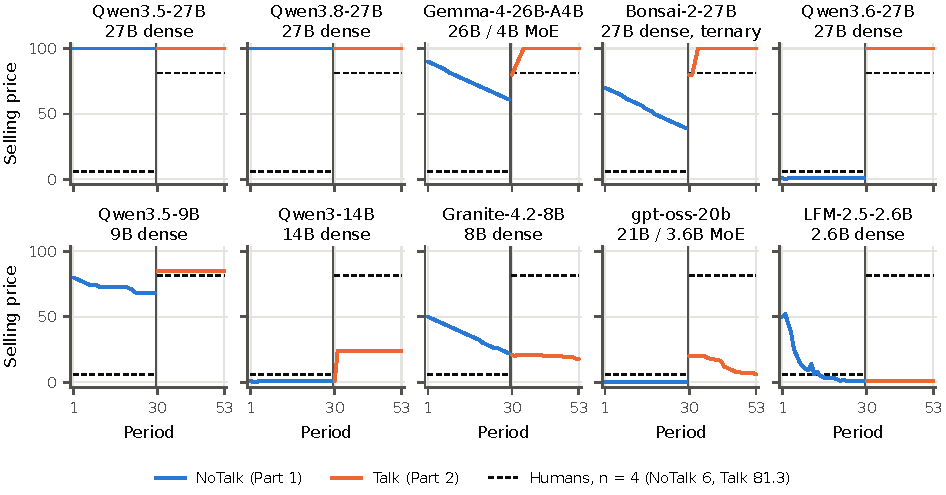
\includegraphics[width=\textwidth]{figures/price-paths.pdf}
\caption{Selling price by period in each model's $n=4$ market (Part 1 NoTalk, periods 1--29; Part 2 Talk, 30--53). Dashed lines: human means (6.0 and 81.3). Panels ordered by Talk price.}
\label{fig:paths}
\end{figure}

\begin{figure}[h]
\centering
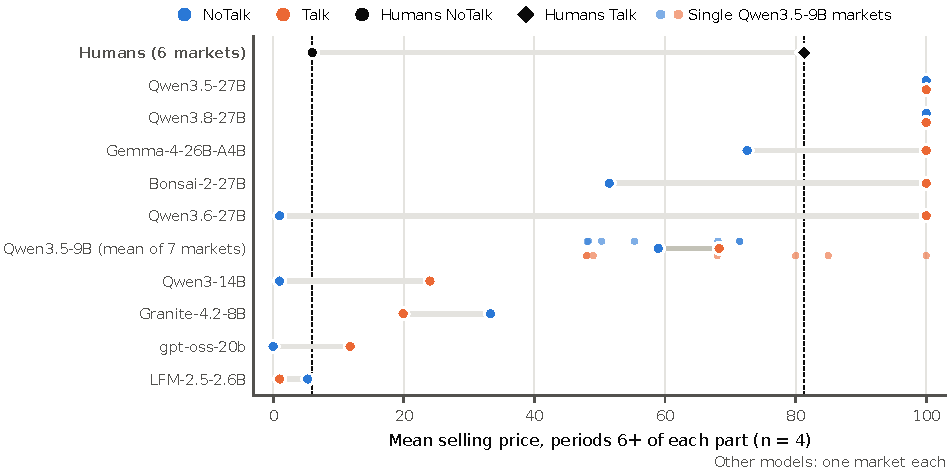
\includegraphics[width=0.85\textwidth]{figures/talk-vs-notalk.pdf}
\caption{NoTalk and Talk selling price (periods 6+) at $n=4$. Qwen3.5-9B shows the mean of 7 markets (faint dots: single markets); all other models have one market.}
\label{fig:dumbbell}
\end{figure}

\begin{figure}[h]
\centering
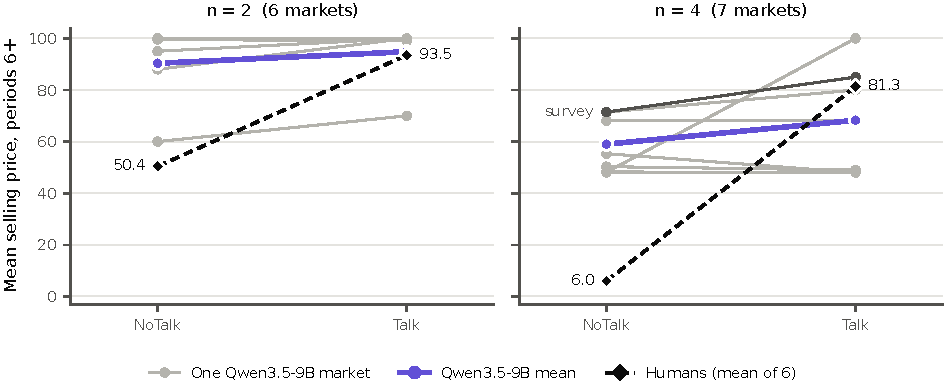
\includegraphics[width=0.85\textwidth]{figures/q35-replication.pdf}
\caption{Qwen3.5-9B replication: NoTalk to Talk selling price per market (grey; the survey market labelled), mean (violet) and human mean (dashed), at $n=2$ (6 markets) and $n=4$ (7 markets).}
\label{fig:repl}
\end{figure}

\clearpage
\begin{thebibliography}{9}
\small
\bibitem{fn2012} M.~A. Fonseca and H.-T. Normann. Explicit vs.\ tacit collusion --- The impact of communication in oligopoly experiments. \emph{European Economic Review} 56(8):1759--1772, 2012. doi:10.1016/j.euroecorev.2012.09.002. Working paper: DICE Discussion Paper No.~65, 2012.
\bibitem{fish} S.~Fish, Y.~A. Gonczarowski and R.~I. Shorrer. Algorithmic collusion by large language models. arXiv:2404.00806.
\bibitem{han} Han, Wu and Xiao. Guinea pig trials. arXiv:2308.10974.
\bibitem{keppo} Keppo, Li, Tsoukalas and Yuan. On the fragility of AI agent collusion. arXiv:2603.20281.
\bibitem{agrawal} Agrawal et al. Evaluating LLM agent collusion in double auctions. ICML 2025, arXiv:2507.01413.
\end{thebibliography}

\end{document}
